%CHAPITRE 9

\chapter{Ajustement d'un modèle $y=f(\vec{x},\vec{a})$ sur une série de mesures}

\section{Introduction}

Admettons que l'on soit en présence d'un circuit de type RLC série avec $R=10$ k$\Omega$ et $L=10$ H mais dont on ne connait pas la valeur de C. Une méthode très précise pour déterminer la valeur de C consiste à mesurer la fonction de transfert courant/tension dans le domaine fréquentiel, et \textbf{d'ajuster} sur cette mesure le modèle de la fonction de transfert, donnée par
\begin{equation}
Y(\omega)=\frac{1}{\sqrt{R^2+\left(\omega L-\frac{1}{\omega C}\right)^2}}
\label{eq:Y}
\end{equation}
L'ajustement consistant, dans le cas présent, à trouver la valeur de C qui \textbf{minimise} l'écart entre modèle et mesures.

Pourquoi considérer tout une gamme de fréquence plutôt qu'une seule mesure à une fréquence donnée ? si nous connaissons en effet $Y$ à une fréquence donnée, nous pourrions très bien utiliser l'équation~\ref{eq:Y} pour en tirer C, et, en utilisant les formules du chapitre précédent, déterminer l'incertitude sur C à partir de l'incertitude sur $Y$. Mais pour que cela fonctionne bien, il faut être certain qu'il n'existe pas d'erreur systématique sur la mesure de $Y$, et que l'erreur aléatoire sur Y soit bien connue.

En réalité, à cause du \textbf{bruit de mesure}, on peut se trouver dans une situation impossible à résoudre~: admettons par exemple que la mesure bruitée de $Y$ soit égale à $1.5\times10^{-4}$, or, il est impossible en théorie que $Y$ soit supérieur à $1/R$ c-à-d $\text{max}(Y)=10^{-4}$. Si on persiste à utiliser cette valeur de $Y$, on tombe sur $\left(\omega L-\frac{1}{\omega C}\right)^2<0$, ce qui est impossible. On voit donc par cet exemple que le bruit peut rendre une mesure unique \textbf{complètement inutile} !

Supposons donc que nous disposions de 20 valeurs bruitées (mais pas trop quand même) de la fonction de transfert $Y$ pour 20 valeurs de $\omega$ de 1 à 20 kHz. Calculons, pour C entre 0.5 nF et 1.5 nF (si on choisit cet intervalle, c'est uniquement parce que l'on pense qu'il contient la valeur optimale de C), l'erreur quadratique totale entre le modèle $Y$ et les 20 mesures,
\begin{equation}
\mathcal{Q}^2(C)=\sum_{i=1}^{20} \left(Y_i-\frac{1}{\sqrt{R^2+\left(\omega_i L-\frac{1}{\omega_i C}\right)^2}}\right)^2
\end{equation}
Le graphique de $\mathcal{Q}^2(C)$ est donné en Fig.~\ref{fig:q2c}. On voit très bien qu'il existe une valeur de $C$ qui minimise $\mathcal{Q}^2(C)$, et cette valeur est $C=1.005$ nF. La même figure montre aussi la superposition des mesures et du modèle optimal de $Y(\omega)$, c-à-d celui associé à la valeur optimale de C.
\begin{figure}[htb]
   \centering
   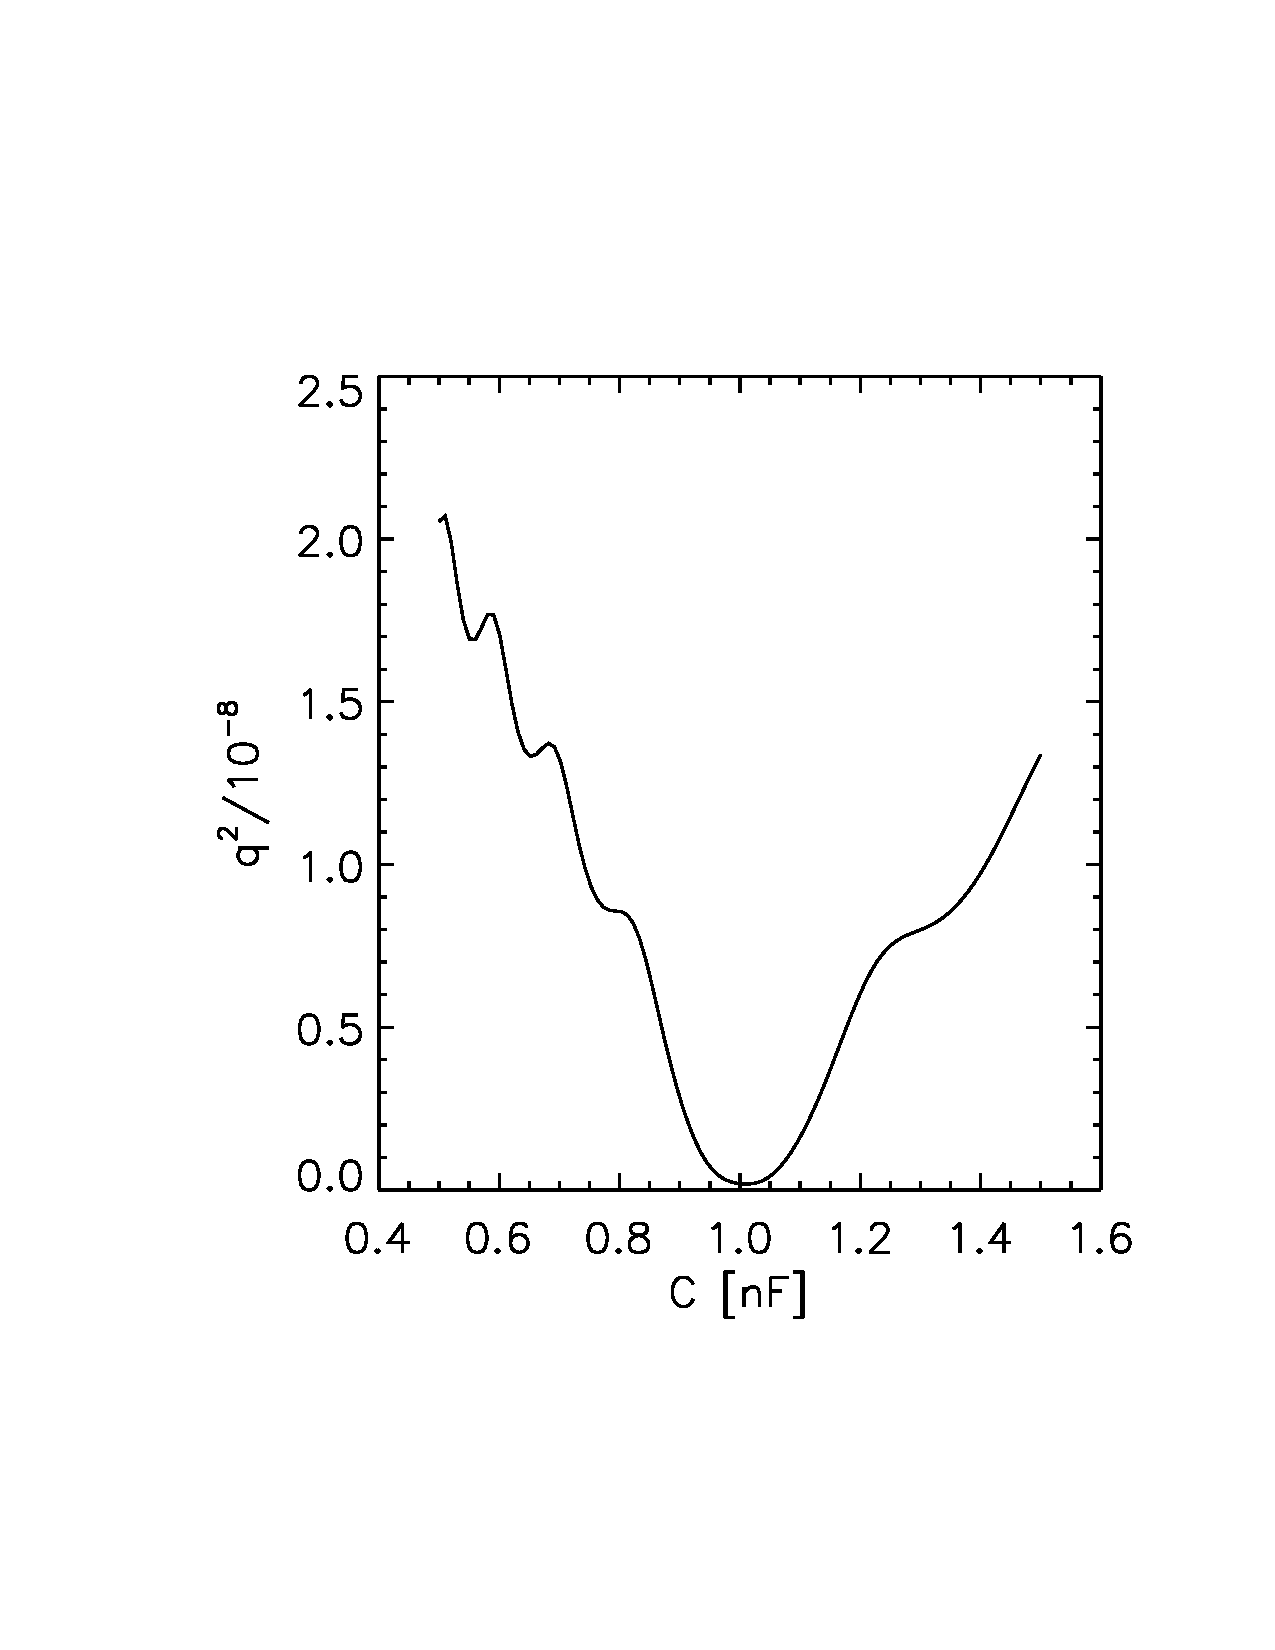
\includegraphics[width=0.45\textwidth]{assets/figures/q2Ymodel.pdf}\hspace{7mm}
   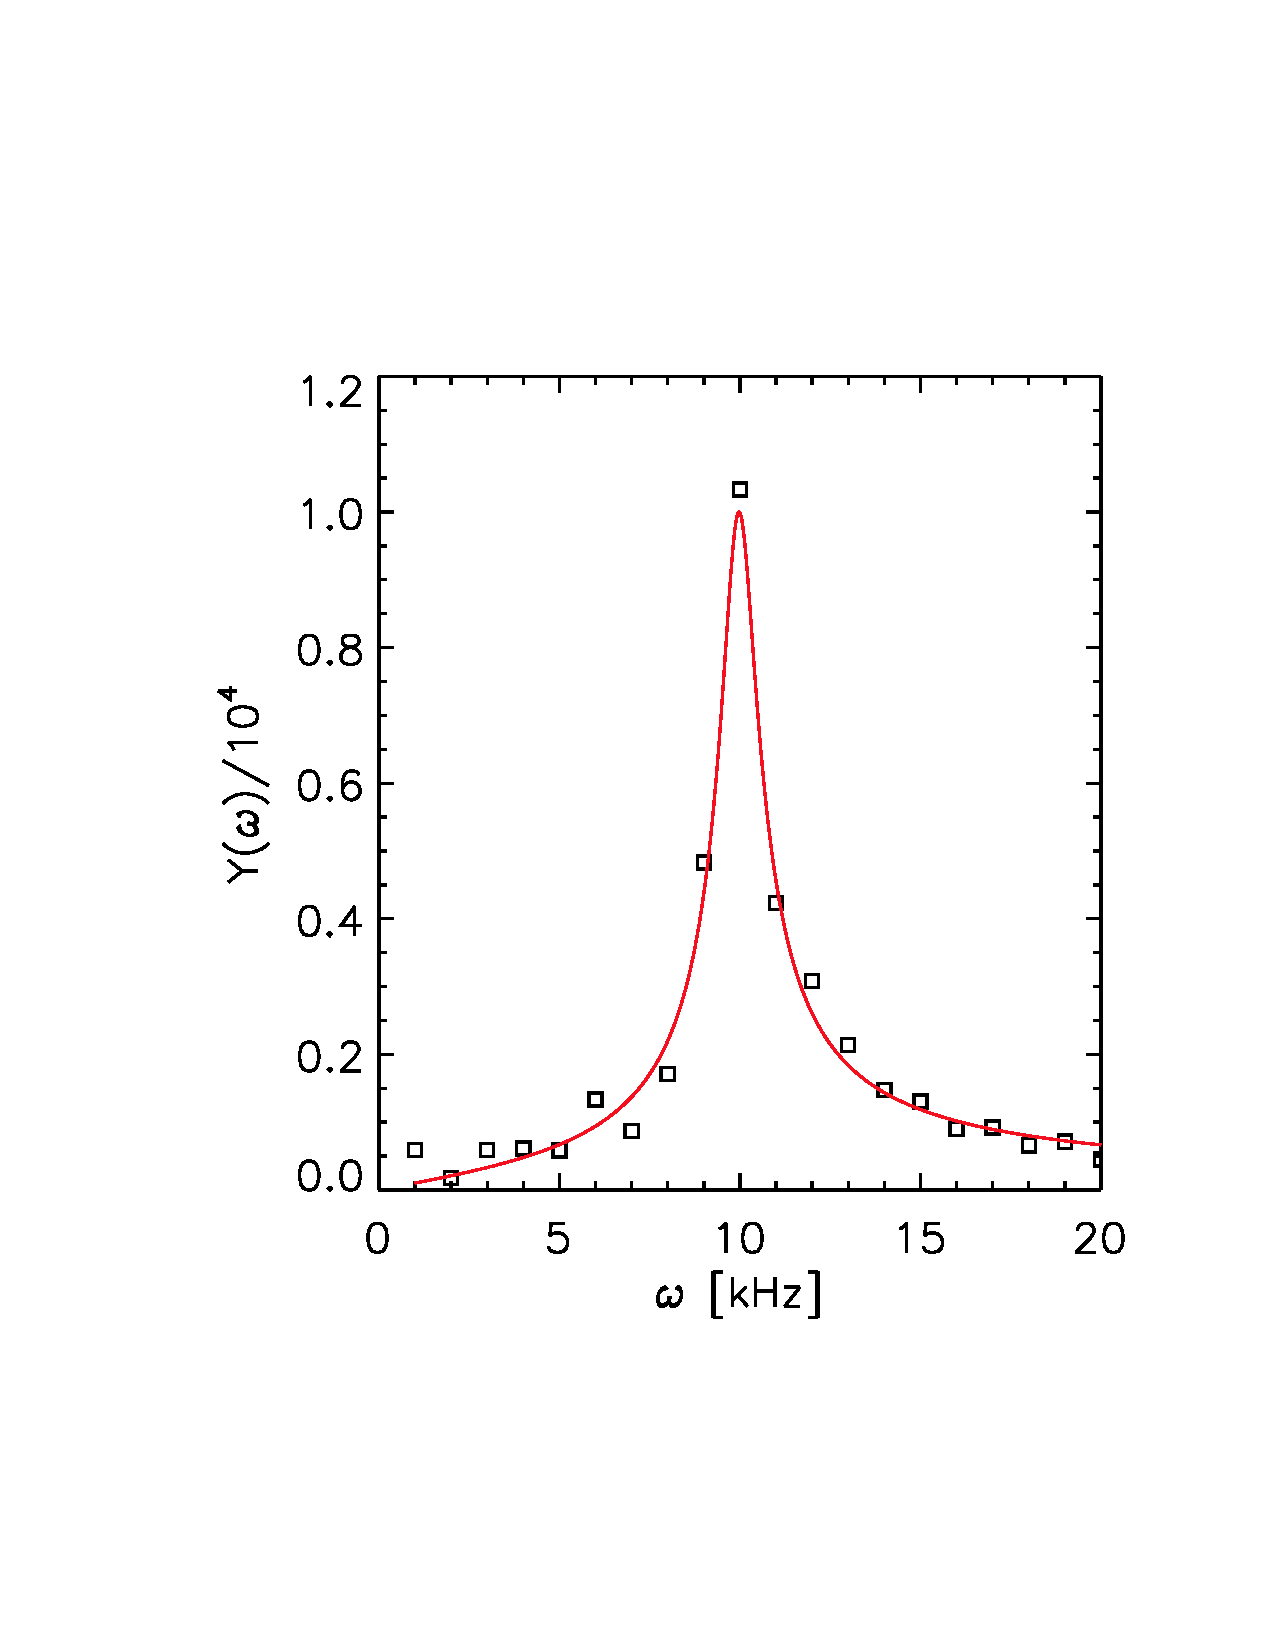
\includegraphics[width=0.45\textwidth]{assets/figures/adjustedModelYtf.pdf}
   \caption{A gauche~: écart quadratique en fonction de la valeur d'essai de C. A droite~: superposition du meilleur modèle $Y(\omega)$, pour $C=1.005$ nF, sur les 20 mesures bruitées.}
   \label{fig:q2c}
\end{figure}

En utilisant N mesures de $Y$ en fonction de N valeurs de $\omega$, on a obtenu autant de mesures indépendantes, qui ont renforcé la validité de la détermination. Les valeurs impossibles de $Y$, dues au bruit, ne posent aucun problème, puisqu'on cherche à minimiser un écart quadratique, donc le signe de l'erreur n'a pas d'importance.

Par ailleurs, la comparaison visuelle des mesures et du modèle permet d'évaluer s'il existe des erreurs systématiques ou aberrantes dans les mesures, et donc de les éliminer. En conclusion, lorsqu'on en a la possibilité, il est \textbf{toujours} préférable de déterminer la valeur d'un paramètre inconnu à travers \textbf{l'ajustement d'un modèle} plutôt que sur une valeur unique.

\section{Théorie}

\begin{wrapfigure}[20]{r}[5pt]{70mm}
   \centering
   \vspace{-5mm}
   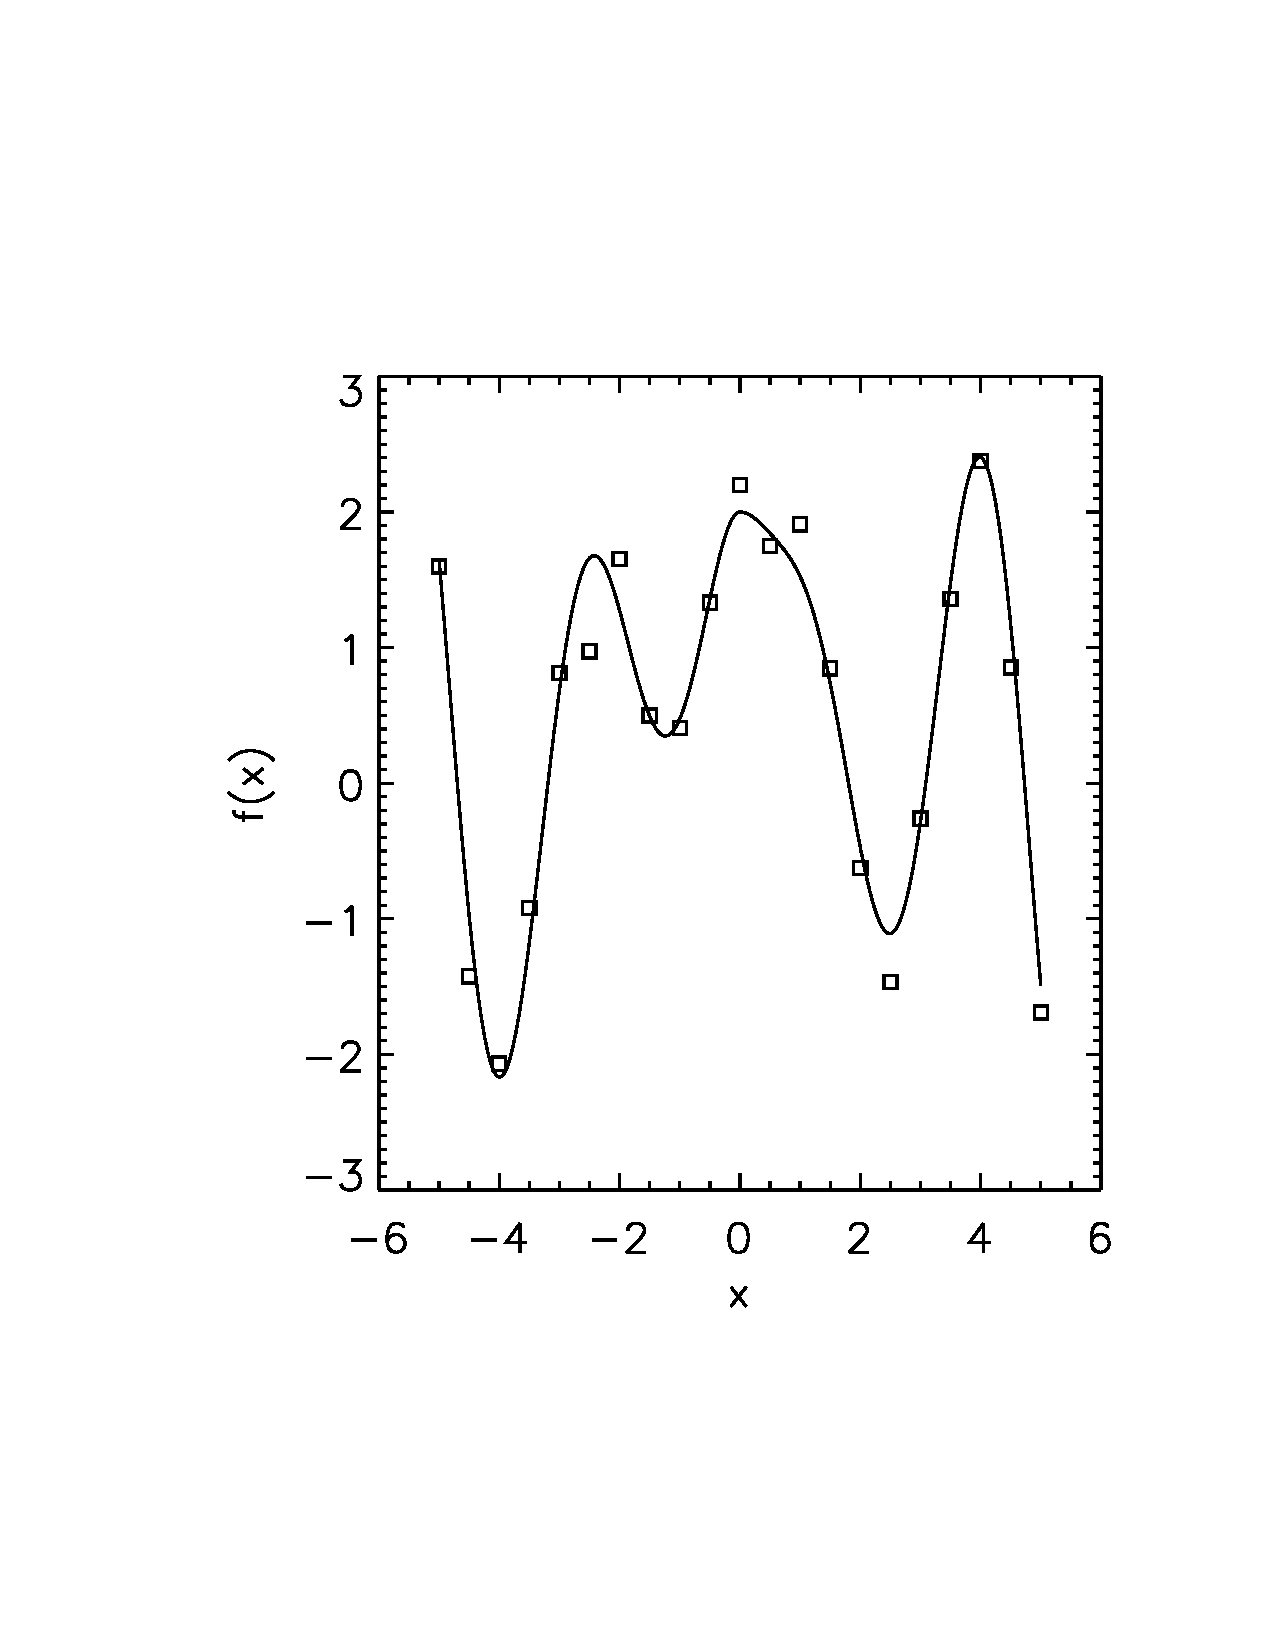
\includegraphics[width=70mm]{assets/figures/exemple1D.pdf}
   \caption{Mesure unidimensionnelle (carrés) et modèle ajusté (courbe continue). Il y a ici 21 couples de mesure $(x_i,y_i)_{i=1\dots 21}$, $N_m=21$.}
   \label{fig:ex1}
\end{wrapfigure}
Soit donc une série de $N_m$ mesures (bruitées ou imprécises) d'une variable $y$ en fonction d'une autre, $x$. La variable $x$ peut être unidimensionnelle, par exemple le temps $t$, ou alors multi-dimensionnelle, comme la position sur un plan, auquel cas $x$ est un vecteur à deux composantes, $\vec{x}=[x_1,x_2]$, ou la position dans un espace, auquel cas $x$ est un vecteur à trois composantes, $\vec{x}=[x_1,x_2,x_3]$. On montre en figure~\ref{fig:ex1} un exemple de mesure \textbf{uni}dimensionnelle.

Notre objectif est de trouver le modèle $y=f(\vec{x},\vec{a})$, muni d'un certain nombre de paramètres $\vec{a}=[a_1,a_2,\dots]$, qui permet de décrire le mieux possible nos mesures. Par exemple, si nous avions la mesure d'un signal sinusoïdal en fonction du temps, et que nous désirions trouver la période de ce signal, il suffirait de chercher la valeur de $T$ telle que le modèle $y(t)=\sin{(2\pi/T)}$ s'ajuste le mieux aux mesures.

Deux cas se présentent dans la pratique~: (1) on connait déjà le modèle sous-jacent aux mesures (par exemple une sinusoïdale comme ci-dessus), ou (2) on ne le connait pas. Dans ce cas, on peut soit chercher (par essais) un modèle qui va bien, ou adopter un modèle polynomial.

Mais dans le cas d'un modèle polynomial, il faut faire attention~: on sait que par 2 points, on peut faire passer une droite, et que par 3 points, un polynôme en $x^2$ etc, donc si on a $N$ points, nous pourrions trouver un polynôme de degré $N-1$ qui passerait par tous les points. Mais cela n'a aucun sens ! en effet, \textbf{toute mesure est bruitée}, c'est-à-dire affectée d'une erreur aléatoire inconnue, par conséquent ajuster un modèle qui passerait par tous les points de mesure équivaut à s'ajuster à du bruit, ce qui conduirait à un modèle polynomial de nos mesures qui ne correspondrait à rien... Par ailleurs, lorsqu'on essaye d'ajuster un polynôme avec exactitude sur trop de points, on aboutit en général à un polynôme avec d'énormes oscillations entre les points, ce qui montre qu'il y a un problème. Donc, on se contentera en général de trouver le degré du polynôme tel que l'écart de l'ajustement soit assez petit, \textit{sans} qu'il y ait d'oscillations.

\subsection{La méthode de la minimisation de l'écart quadratique entre modèle et mesures}

Admettons donc que nous ayons choisi un modèle avec paramètres, $y=f(\vec{x},\vec{a})$, censé décrire nos mesures. Par exemple, le modèle associé aux mesures de la fig.~\ref{fig:ex1} est le suivant~:
\begin{equation}
f(x,\vec{a})=\,\frac{x\,\sin{a_1x}}{a_2}+\frac{a_3}{x^2+a_4}
\end{equation}
et les valeurs des paramètres utilisés dans le cas particulier de la fig.~\ref{fig:ex1} sont $\vec{a}=[2,1.73,2,1]$. En principe, on ne possède que la forme générale de la fonction $f(\vec{x},\vec{a})$, mais on ne connait pas les valeurs des paramètres.

\begin{center}
\fbox{
\begin{minipage}{0.95\textwidth}\textbf{Ajuster le modèle $f(\vec{x},\vec{a})$, en pratique, c'est trouver les valeurs des paramètres $\vec{a}=[a_1,a_2,\dots]$ telles que l'écart entre le modèle et les mesures, aux coordonnées $\vec{x}_i$ des points de mesures, soit le plus petit possible}.
\end{minipage}
}
\end{center}

Mathématiquement, on va \textit{définir} l'écart $\mathcal{Q}^2$ par la somme, sur les $N_m$ points de mesure, des écarts individuels, au carré, entre le modèle $f(\vec{x}_i,\vec{a})$, au point de coordonnées $\vec{x}_i$, et la mesure $y_i$, soit
\begin{equation}
\mathcal{Q}^2(\vec{a})=\sum\limits_{i=1}^{N_m}\big[f(\vec{x}_i,\vec{a})-y_i\big]^2
\end{equation}
et on a considéré le carré de l'écart, car puisque nous sommes intéressé à mesurer une distance entre points de mesure et modèle, il nous faut prendre une mesure de l'écart qui soit toujours positive. Nous aurions aussi pu considérer la valeur absolue de l'écart, mais les développement mathématiques que l'on va voir dans la suite auraient étés plus complexes. En revanche, il ne faudrait surtout pas considérer l'écart simple, car la somme des écarts simples ne peut pas être minimisée : elle peut être nulle, sans que la valeur des paramètres soit optimale.

\newpage
\begin{figure}[h!]
   \centering
   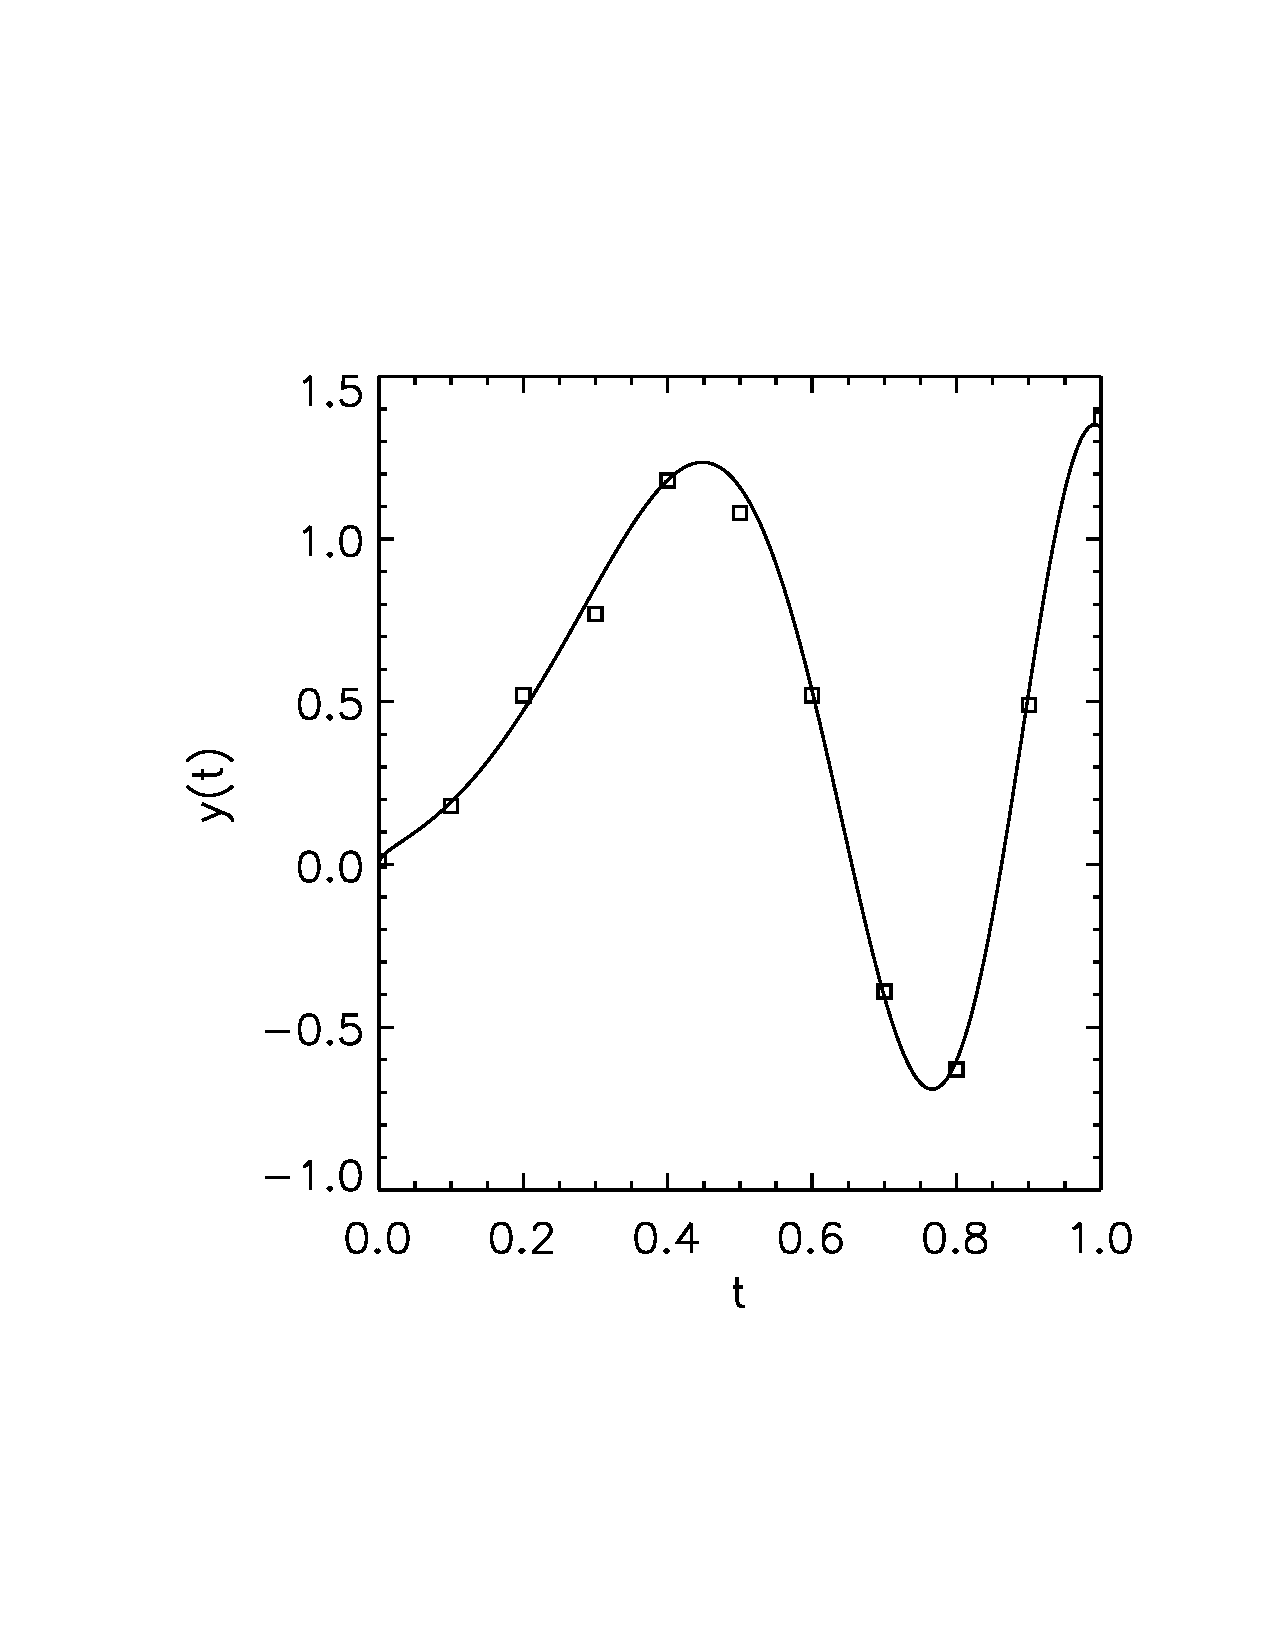
\includegraphics[height=6.5cm]{assets/figures/prob4.pdf}\hspace{1cm}
   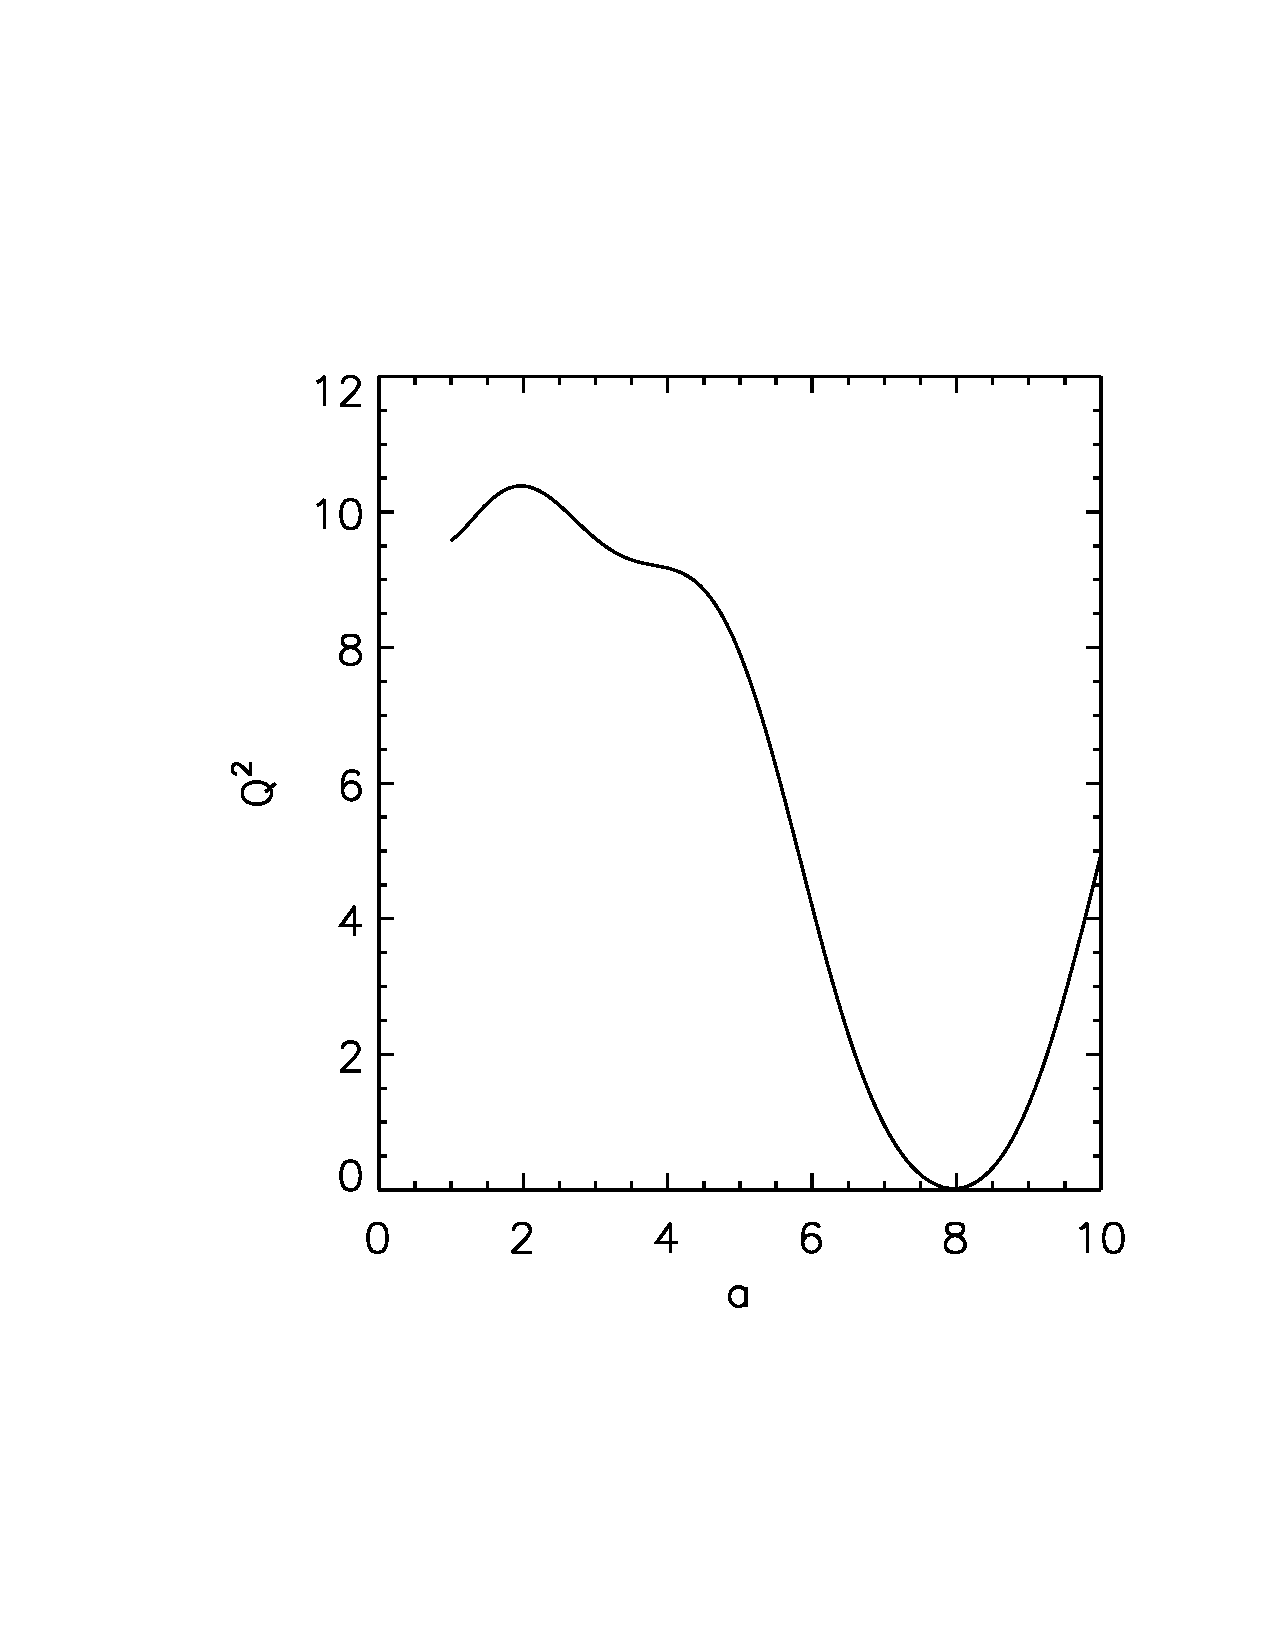
\includegraphics[height=6.5cm]{assets/figures/figure2.pdf}
   \caption{A gauche~: points de mesure (carrés) et modèle; à droite~: écart quadratique $\mathcal{Q}^2(a)$ en fonction du paramètre $a$.}
   \label{fig:q2a}
\end{figure}
Considérons, pour illustrer notre propos, le cas d'un modèle simple à 1 seul paramètre. On a les 11 points de mesure suivants (voir figure~\ref{fig:q2a})~:
\begin{center}
\begin{tabular}{r|ccccccccccc}
$t_i$ & 0 & 0.1 & 0.2 & 0.3 & 0.4 & 0.5 & 0.6 & 0.7 & 0.8 & 0.9 & 1 \\
$y_i$ & 0.01 & 0.18 & 0.52 & 0.77 & 1.18 & 1.08 & 0.52 & -0.39 & -0.63 & 0.49 & 1.37
\end{tabular}
\end{center}
auxquels on désire ajuster le modèle à un seul paramètre suivant~:
$$
y(t)=\sqrt{\frac{t}{a}}+\sin{(a t^2)}
$$
Il s'agit donc de trouver la valeur de $a$ qui donne le meilleur ajustement du modèle aux données. Calculons (il faut programmer un peu, sous MATLAB) l'écart quadratique en fonction de $a$ pour un intervalle de $a$ - choisi un peu au hasard - entre 1 et 10. Le graphique de $\mathcal{Q}^2(a)$ est donné en figure~\ref{fig:q2a}, et on voit clairement qu'il existe une valeur de $a$ optimale autour de 8 (avec $\mathcal{Q}^2(8)=0.019$). Ici, le minimum est très marqué, mais dans certains cas, il peut l'être un peu moins, en particulier en présence de grandes erreurs de mesures : dans ce cas, même avec la valeur correcte du paramètre, l'écart entre modèle et mesure pourra être grand, et sera donné par la somme (quadratique) des erreurs de mesure.

Par essais successifs, en restreignant l'intervalle de recherche de $a$ autour de la valeur minimale, on trouve que la valeur optimale de $a$ converge vers 7.9613725. En réalité, la valeur de $a$ qui fut utilisée pour la construction du modèle est 8, exactement. On voit donc ici l'effet du bruit de la mesure : la valeur optimale n'est pas toujours la "vraie" valeur ! Avec un calcul d'erreur, cependant, on arriverait à calculer une incertitude sur la détermination de $a$, en fonction des incertitudes sur les mesures - mais ce n'est pas le propos de ce document.

Lorsqu'il y a plus que 1 paramètre, il suffit d'effectuer le calcul de $\mathcal{Q}^2$ sur des intervalles bien choisis pour l'ensemble des paramètres, et de déterminer les valeurs des paramètres où $\mathcal{Q}^2$ est minimum (fond de la vallée d'une carte en $a_1,a_2$ pour un problème à deux paramètres, etc.)

\subsection{Soyons plus malins, et utilisons la dérivée !}

En effet, le minimum de la courbe $\mathcal{Q}^2(a)$, qui nous donne le lieu de la solution optimale, peut se trouver facilement, sans faire de calculs numériques (ni programmation) en calculant analytiquement la dérivée de $\mathcal{Q}^2(a)$ par rapport à $a$, et en posant = 0. On trouve une équation en $a$ dont la solution est forcément la valeur optimale de $a$. Parfois, il y a plusieurs solutions à l'équation de la dérivée, et une de ces solutions peut en fait indiquer un \textit{maximum} de $\mathcal{Q}^2(a)$, ou un \textbf{minimum local}, comme on peut le voir sur les Figs.~\ref{fig:q2c} ou~\ref{fig:q2a}, donc il faut toujours être un peu prudent et vérifier si on a trouvé la bonne solution - en général, cependant, on tombe souvent sur le minimum de $\mathcal{Q}^2(a)$.

Dans le cas où on a un vecteur de paramètres $\vec{a}$ (disons de dimension $M$, donc $M$ paramètres), il suffit de calculer une dérivée pour chaque $a_{k=1\dots M}$, et on se retrouve avec un système de $M$ équations à $M$ inconnues. Donc, en principe, on a tout ce qu'il faut pour trouver les valeurs optimales des paramètres.

Mais il y a parfois une difficulté. Il se peut, pour certains modèles, que les $M$ équations ne soient pas du tout simples à transformer en formules donnant directement les valeurs optimales du vecteur $\vec{a}$. Dans ce cas, on est un peu obligé de retourner à une recherche numérique, comme dans l'exemple de la figure~\ref{fig:q2a}.

Ignorons cependant ce problème éventuel, et examinons le cas où $f(\vec{x},\vec{a})$ est une relation linéaire en $\vec{a}$,
\begin{equation}
f(\vec{x},\vec{a})=a_1f_1(\vec{x})+a_2f_2(\vec{x})+a_3f_3(\vec{x})+\dots+a_Mf_M(\vec{x})
\label{eq:eq03}
\end{equation}
Les fonctions $f_{k=1\dots M}$ peuvent être ce que l'on veut (quelconques), la seule chose qui compte est que ces fonctions ne contiennent aucun des paramètres $a_k$.

Minimisons l'écart quadratique total entre les données et le modèle, en posant que la dérivée de cet écart par rapport à chacun des paramètres $a_{k=1\dots M}$ est nulle,
\begin{equation}
\frac{\partial}{\partial a_k}\sum\limits_{i=1}^{N_m}\big[f(\vec{x}_i,\vec{a})-y_i\big]^2=0
\end{equation}
en développant, on trouve un système de $M$ équations,
\begin{equation}
\sum\limits_{i=1}^{N_m}\frac{\partial f(\vec{x}_i,\vec{a})}{\partial a_j}f(\vec{x}_i,\vec{a})=
\sum\limits_{i=1}^{N_m}\frac{\partial f(\vec{x}_i,\vec{a})}{\partial a_j}y_i
\end{equation}
Puisque l'on a $M$ équations en $\vec{a}$, on peut en extraire à priori les $M$ paramètres inconnus. Avec l'équation~(\ref{eq:eq03}), il est facile de voir que le système des $M$ équations devient
\begin{eqnarray}
\frac{\partial }{\partial a_1} \text{:} &
\sum\limits_{k=1}^{M}\sum\limits_{i=1}^{N_m}a_k\,f_1(\vec{x}_i)\,f_j(\vec{x}_i)=
\sum\limits_{i=1}^{N_m}f_1(\vec{x}_i)\,y_i\\\nonumber
\frac{\partial }{\partial a_2} \text{:} &
\sum\limits_{k=1}^{M}\sum\limits_{i=1}^{N_m}a_k\,f_2(\vec{x}_i)\,f_j(\vec{x}_i)=
\sum\limits_{i=1}^{N_m}f_2(\vec{x}_i)\,y_i\\\nonumber
& \vdots\\\nonumber
\frac{\partial }{\partial a_{M}} \text{:} &
\sum\limits_{k=1}^{M}\sum\limits_{i=1}^{N_m}a_k\,f_{M}(\vec{x}_i)\,f_j(\vec{x}_i)=
\sum\limits_{i=1}^{N_m}f_{M}(\vec{x}_i)\,y_i\\\nonumber
\end{eqnarray}
et si on détaille les deux premières et la dernière des équations,
\begin{gather}
a_1\sum\limits_{i=1}^{N_m}f_1^2(\vec{x}_i)+
a_2\sum\limits_{i=1}^{N_m}f_2(\vec{x}_i)\,f_1(\vec{x}_i)+
\cdots
a_{M}\sum\limits_{i=1}^{N_m}f_{M}(\vec{x}_i)\,f_1(\vec{x}_i)=
\sum\limits_{i=1}^{N_m}f_1(\vec{x}_i)\,y_i\\\nonumber
a_1\sum\limits_{i=1}^{N_m}f_1(\vec{x}_i)\,f_2(\vec{x}_i)+
a_2\sum\limits_{i=1}^{N_m}f_2^2(\vec{x}_i)+
\cdots
a_{M}\sum\limits_{i=1}^{N_m}f_{M}(\vec{x}_i)\,f_2(\vec{x}_i)=
\sum\limits_{i=1}^{N_m}f_2(\vec{x}_i)\,y_i\\\nonumber
\vdots\\\nonumber
a_1\sum\limits_{i=1}^{N_m}f_1(\vec{x}_i)\,f_M(\vec{x}_i)+
a_2\sum\limits_{i=1}^{N_m}f_2(\vec{x}_i)\,f_M(\vec{x}_i+
\cdots
a_{M}\sum\limits_{i=1}^{N_m}f_{M}^2(\vec{x}_i)=
\sum\limits_{i=1}^{N_m}f_M(\vec{x}_i)\,y_i\nonumber
\end{gather}
on comprend vite alors que l'on peut écrire ce système sous la forme d'un produit de matrices,
\begin{equation}
\begin{bmatrix}
\sum_i f_1^2(\vec{x}_i)       & \sum_i f_2(\vec{x}_i)f_1(\vec{x}_i) & \cdots & \sum_i f_{M}(\vec{x}_i)f_1(\vec{x}_i)\\
\sum_i f_1(\vec{x}_i)f_2(\vec{x}_i) & \sum_i f_2^2(\vec{x}_i)       & \cdots & \sum_i f_{M}(\vec{x}_i)f_2(\vec{x}_i)\\
\vdots & \vdots & \vdots & \vdots \\
\sum_i f_1(\vec{x}_i)f_{M}(\vec{x}_i) & \sum_i f_2(\vec{x}_i)f_{M}(\vec{x}_i) & \cdots & \sum_i f_{M}^2(\vec{x}_i)
\end{bmatrix}
\begin{bmatrix} a_1 \\ a_2 \\ \vdots \\ a_{M}\end{bmatrix}=
\begin{bmatrix}
\sum_if_1(\vec{x}_i)\,y_i\\
\sum_if_2(\vec{x}_i)\,y_i\\
\vdots\\
\sum_if_{M}(\vec{x}_i)\,y_i
\end{bmatrix}\label{eq:emplrdp}
\end{equation}
ou
\begin{equation}
A\cdot\vec{a}=\vec{b}
\end{equation}
La matrice $A$ et le vecteur $\vec{b}$ se calculent numériquement à partir de la connaissance des fonctions $f_j(x)$ et des points de mesure $(\vec{x}_i,y_i)$. La solution est donnée par
\begin{equation}
\vec{a}=A^{-1}\cdot\vec{b}
\end{equation}

\section{Application~: ajustement d'une droite $y=ax+b$ et lien avec la corrélation linéaire}

Très souvent dans la pratique on observe des processus linéaires ou facilement linéarisables, c-à-d pouvant se ramener à une droite $y=mx+p$, $x$ et $y$ étant les mesures et $m$ et $p$ les paramètres inconnus que l'on cherche. Par exemple la décharge d'un condensateur s'exprime par une relation exponentielle $u(t)=u_0\exp{-kt}$ où $1/k$ est la constante de temps du condensateur. En mesurant $u$ pour une série de valeurs de $t$, et en calculant le log naturel de $u$ on obtient la relation linéarisée $\ln{u}=\ln{u_0}-kt$. En ajustant une droite sur les points de mesure $\ln{u_i}$ et $t_i$ on va pouvoir trouver $u_0$ et la constante de temps $1/k$.

Appliquons donc la théorie de l'ajustement ci-dessus au cas de la droite $y=mx+p$. On a $a_1=m$ et $a_2=p$, ainsi que $f_1(x)=x$ et $f_2(x)=1$ (une constante). Les éléments de la matrice de l'équation~\ref{eq:emplrdp} sont les suivants, avec $N$ le nombre de mesures,
\begin{equation}
A=
\begin{bmatrix}
\sum_i^N f_1^2(x_i) & \sum_i^N f_2(x_i)f_1(x_i)\\
\sum_i^N f_1(x_i)f_{2}(x_i) & \sum_i^N f_{2}^2(x_i)
\end{bmatrix}=
\begin{bmatrix}
\sum_i^N x_i^2 & \sum_i^N x_i\\
\sum_i^N x_i & N
\end{bmatrix}
\end{equation}
le vecteur $\vec{a}$ est simplement
\begin{equation}
\vec{a}=
\begin{bmatrix}
m \\ p
\end{bmatrix}
\end{equation}
et le vecteur $\vec{b}$ est
\begin{equation}
\vec{b}=
\begin{bmatrix}
\sum_i^N x_iy_i \\ \sum_i^N y_i
\end{bmatrix}
\end{equation}
On a donc à résoudre le système simple
\begin{equation}
\begin{bmatrix}
\sum_i^N x_i^2 & \sum_i^N x_i\\
\sum_i^N x_i & N
\end{bmatrix}
\begin{bmatrix}
m \\ p
\end{bmatrix}
=
\begin{bmatrix}
\sum_i^N x_iy_i \\ \sum_i^N y_i
\end{bmatrix}
\end{equation}
dont la solution est (à vérifier vous-même)
\begin{gather}
m=\frac{\sigma_y}{\sigma_x}\,\Gamma(x,y)\\
p=\langle y\rangle-m\langle y\rangle
\end{gather}
Nous obtenons donc un lien direct entre corrélation et pente de la droite de meilleur ajustement. Voir les exercices pour des exemples.

\section{Un exemple complet en deux dimensions}

Soit la mesure de la cote d'une surface (plus ou moins) plane, en 150 points de coordonnées $\vec{x}=[x,y]_{i=1\dots 150}$. Les points sont mesurés sur une grille de 15-par-10 éléments, la première composante $x$ est la coordonnée horizontale,
\begin{center}
\begin{tabular}{ccccccccccccccc}
1 & 2 & 3 & 4 & 5 & 6 & 7 & 8 & 9 & 10 & 11 & 12 & 13 & 14 & 15 \\
1 & 2 & 3 & 4 & 5 & 6 & 7 & 8 & 9 & 10 & 11 & 12 & 13 & 14 & 15 \\
1 & 2 & 3 & 4 & 5 & 6 & 7 & 8 & 9 & 10 & 11 & 12 & 13 & 14 & 15 \\
1 & 2 & 3 & 4 & 5 & 6 & 7 & 8 & 9 & 10 & 11 & 12 & 13 & 14 & 15 \\
1 & 2 & 3 & 4 & 5 & 6 & 7 & 8 & 9 & 10 & 11 & 12 & 13 & 14 & 15 \\
1 & 2 & 3 & 4 & 5 & 6 & 7 & 8 & 9 & 10 & 11 & 12 & 13 & 14 & 15 \\
1 & 2 & 3 & 4 & 5 & 6 & 7 & 8 & 9 & 10 & 11 & 12 & 13 & 14 & 15 \\
1 & 2 & 3 & 4 & 5 & 6 & 7 & 8 & 9 & 10 & 11 & 12 & 13 & 14 & 15 \\
1 & 2 & 3 & 4 & 5 & 6 & 7 & 8 & 9 & 10 & 11 & 12 & 13 & 14 & 15 \\
1 & 2 & 3 & 4 & 5 & 6 & 7 & 8 & 9 & 10 & 11 & 12 & 13 & 14 & 15
\end{tabular}
\end{center}
la seconde composante, $y$, la coordonnée verticale,
\begin{center}
\begin{tabular}{ccccccccccccccc}
1 & 1 & 1 & 1 & 1 & 1 & 1 & 1 & 1 & 1 & 1 & 1 & 1 & 1 & 1\\
2 & 2 & 2 & 2 & 2 & 2 & 2 & 2 & 2 & 2 & 2 & 2 & 2 & 2 & 2\\
3 & 3 & 3 & 3 & 3 & 3 & 3 & 3 & 3 & 3 & 3 & 3 & 3 & 3 & 3\\
4 & 4 & 4 & 4 & 4 & 4 & 4 & 4 & 4 & 4 & 4 & 4 & 4 & 4 & 4\\
5 & 5 & 5 & 5 & 5 & 5 & 5 & 5 & 5 & 5 & 5 & 5 & 5 & 5 & 5\\
6 & 6 & 6 & 6 & 6 & 6 & 6 & 6 & 6 & 6 & 6 & 6 & 6 & 6 & 6\\
7 & 7 & 7 & 7 & 7 & 7 & 7 & 7 & 7 & 7 & 7 & 7 & 7 & 7 & 7\\
8 & 8 & 8 & 8 & 8 & 8 & 8 & 8 & 8 & 8 & 8 & 8 & 8 & 8 & 8\\
9 & 9 & 9 & 9 & 9 & 9 & 9 & 9 & 9 & 9 & 9 & 9 & 9 & 9 & 9\\
10 & 10 & 10 & 10 & 10 & 10 & 10 & 10 & 10 & 10 & 10 & 10 & 10 & 10 & 10
\end{tabular}
\end{center}
et les cotes mesurées en ces points sont les suivantes (en $\mu$m), avec une erreur aléatoire,
\begin{center}
\begin{tabular}{ccccccccccccccc}
14 & 33 & -35 & 6 & -5 & -2 & 5 & 30 & -6 & 17 & -8 & 7 & -14 & 39 & 12\\
32 & 9 & 65 & 34 & 1 & 20 & 38 & 62 & 40 & 90 & 22 & 83 & 47 & 114 & 82\\
45 & 52 & 69 & 65 & 91 & 99 & 94 & 84 & 104 & 75 & 149 & 174 & 138 & 194 & 194\\
97 & 91 & 73 & 144 & 72 & 139 & 154 & 186 & 141 & 220 & 173 & 195 & 209 & 227 & 247\\
87 & 119 & 155 & 147 & 174 & 157 & 186 & 224 & 213 & 226 & 246 & 333 & 291 & 298 & 341\\
126 & 152 & 156 & 174 & 208 & 222 & 250 & 235 & 295 & 302 & 295 & 320 & 341 & 401 & 399\\
160 & 168 & 186 & 234 & 242 & 280 & 270 & 316 & 355 & 383 & 369 & 402 & 432 & 457 & 456\\
161 & 189 & 196 & 237 & 277 & 313 & 356 & 335 & 381 & 371 & 412 & 459 & 471 & 536 & 586\\
172 & 241 & 261 & 285 & 311 & 315 & 358 & 415 & 429 & 487 & 431 & 535 & 604 & 646 & 672\\
214 & 248 & 276 & 296 & 321 & 322 & 429 & 458 & 474 & 499 & 597 & 566 & 619 & 664 & 698
\end{tabular}
\end{center}
On désire ajuster à ces mesures de cotes le modèle ci-dessous, d'ordre 2,
\begin{equation}
f(\vec{x},\vec{a})=a_1+a_2\,x+a_3\,y+a_4\,x^2+a_5\,x\,y+a_6\,y^2
\end{equation}
Il y a donc 6 paramètres, $\vec{a}=[a_1,a_2,a_3,a_4,a_5,a_6]$, et 6 fonctions $f_k(\vec{x})$,
\begin{gather}
f_1(x,y)=1\\
f_2(x,y)=x\\
f_3(x,y)=y\\
f_4(x,y)=x^2\\
f_5(x,y)=x\,y\\
f_6(x,y)=y^2
\end{gather}
La matrice $A$, de dimension 6-par-6, s'écrit (et on enlève les signes $\sum_i$ pour alléger la notation)
\begin{equation}
A=
\begin{bmatrix}
N_m    & x_i        & y_i        & x_i^2        & x_i\,y_i     & y_i^2 \\
x_i    & x_i^2      & y_i\,x_i   & x_i^3        & x_i^2\,y_i   & y_i^2\,x_i \\
y_i    & x_i\,y_i   & y_i^2      & x_i^2\,y_i   & x_i\,y_i^2   & y_i^3 \\
x_i^2  & x_i^3      & y_i\,x_i^2 & x_i^4        & x_i^3\,y_i   & y_i^2\,x_i^2 \\
x_i\,y_i & x_i^2\,y_i & y_i^2\,x_i & x_i^3\,y_i   & x_i^2\,y_i^2 & y_i^3\,x_i \\
y_i^2  & x_i\,y^2   & y_i^3      & x_i^2\,y_i^2 & x_i\,y_i^3   & y_i^4
\end{bmatrix}
\end{equation}
et le vecteur $\vec{b}$, où $m_i$ sont les mesures aux 150 points,
\begin{equation}
\vec{b}=
\begin{bmatrix}
m_i\\
x_i\,m_i\\
y_i\,m_i\\
x_i^2\,m_i\\
x_i\,y_i\,m_i\\
y_i^2\,m_i
\end{bmatrix}
\end{equation}
Numériquement, on trouve
\begin{equation}
A=
\begin{bmatrix}
    150 &   1200 &   825 &   12400 &   6600 &   5775 \\
   1200 &  12400 &  6600 &  144000 &  68200 &  46200 \\
    825 &   6600 &  5775 &   68200 &  46200 &  45375 \\
  12400 & 144000 & 68200 & 1783120 & 792000 & 477400 \\
   6600 &  68200 & 46200 &  792000 & 477400 & 363000 \\
   5775 &  46200 & 45375 &  477400 & 363000 & 379995
\end{bmatrix}
\vec{b}=
\begin{bmatrix}
  34733 \\
 328927 \\
 252643 \\
3701227 \\
2392112 \\
2010973
\end{bmatrix}
\end{equation}
et les paramètres d'ajustement optimal sont données par
\begin{equation}
\vec{a}=A^{-1}\cdot\vec{b}=
\begin{bmatrix}
-13.3 \\
-8.2 \\
24.1 \\
0.31 \\
3.9 \\
-0.50
\end{bmatrix}
\ \ \text{alors que les vraies valeurs sont}\ \ \vec{a}_{\text{init}}=
\begin{bmatrix}
0 \\
-10 \\
20 \\
0.4 \\
4 \\
-0.2
\end{bmatrix}
\end{equation}
La solution, hormis le premier coefficient, est assez proche des valeurs des paramètres qui furent utilisés lors de la construction des données, et la différence s'explique par le fait qu'un bruit aléatoire fut ajouté aux données simulées. On montre en fig.~\ref{fig:dmr} la carte de la cote mesurée, le modèle, et le résidu de l'ajustement, essentiellement dû au bruit (erreur) de mesure.
\begin{figure}[p]
   \centering
   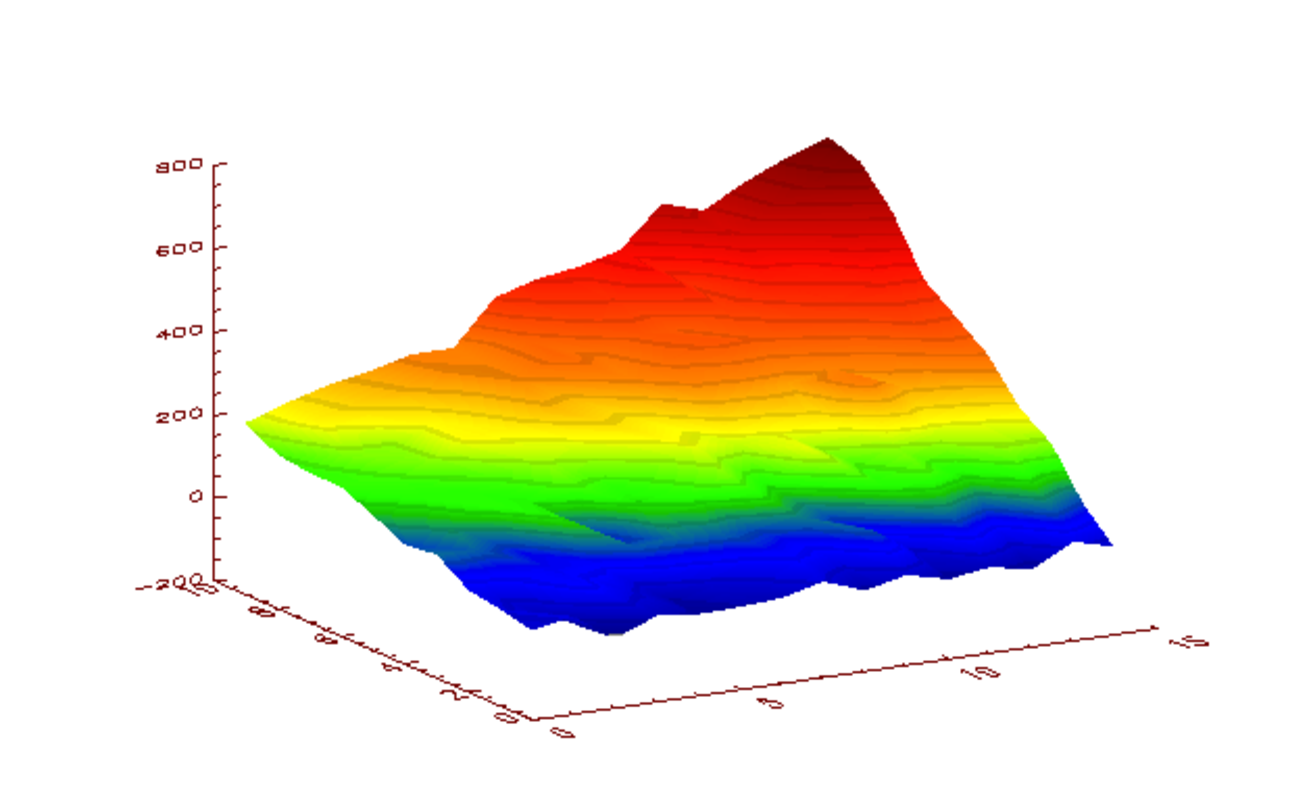
\includegraphics[width=9.3cm]{assets/figures/exempleData.pdf}\vspace{5mm}
   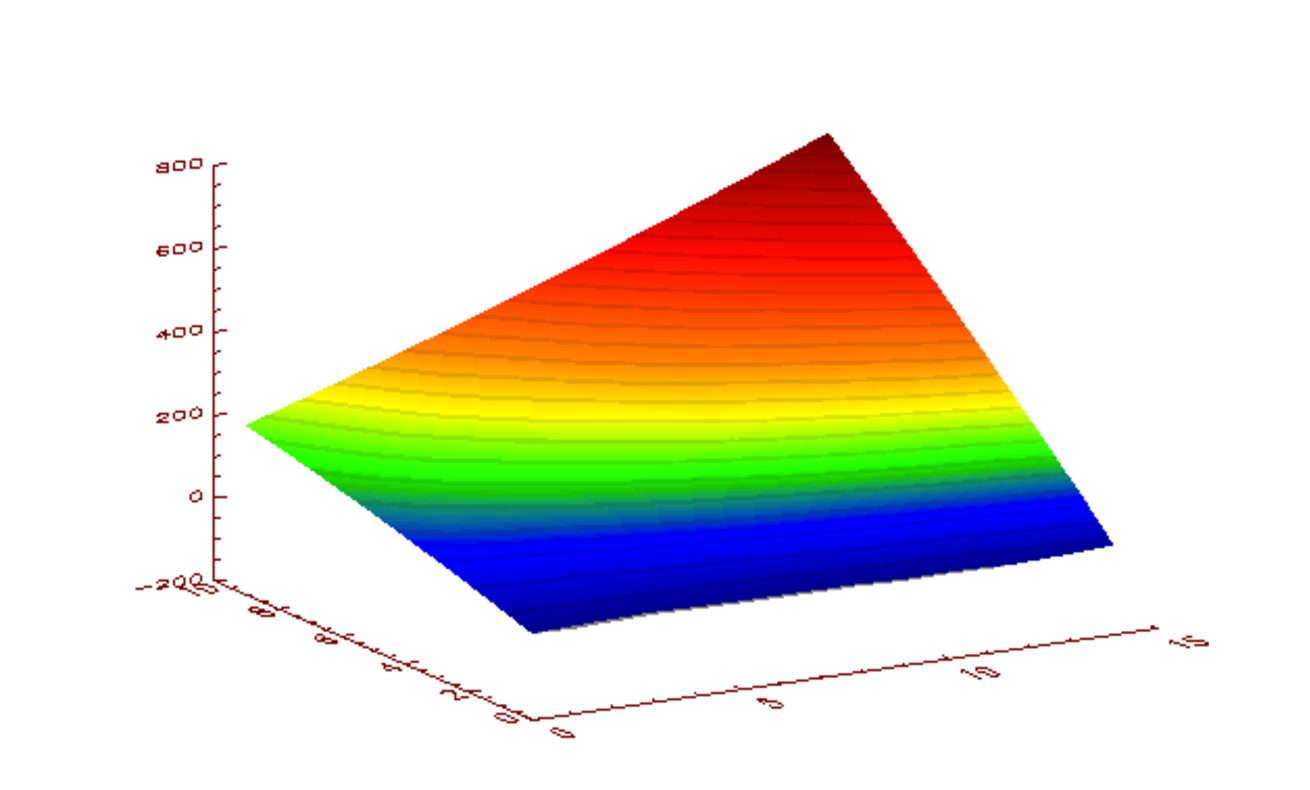
\includegraphics[width=9.3cm]{assets/figures/exempleModel.pdf}\vspace{5mm}
   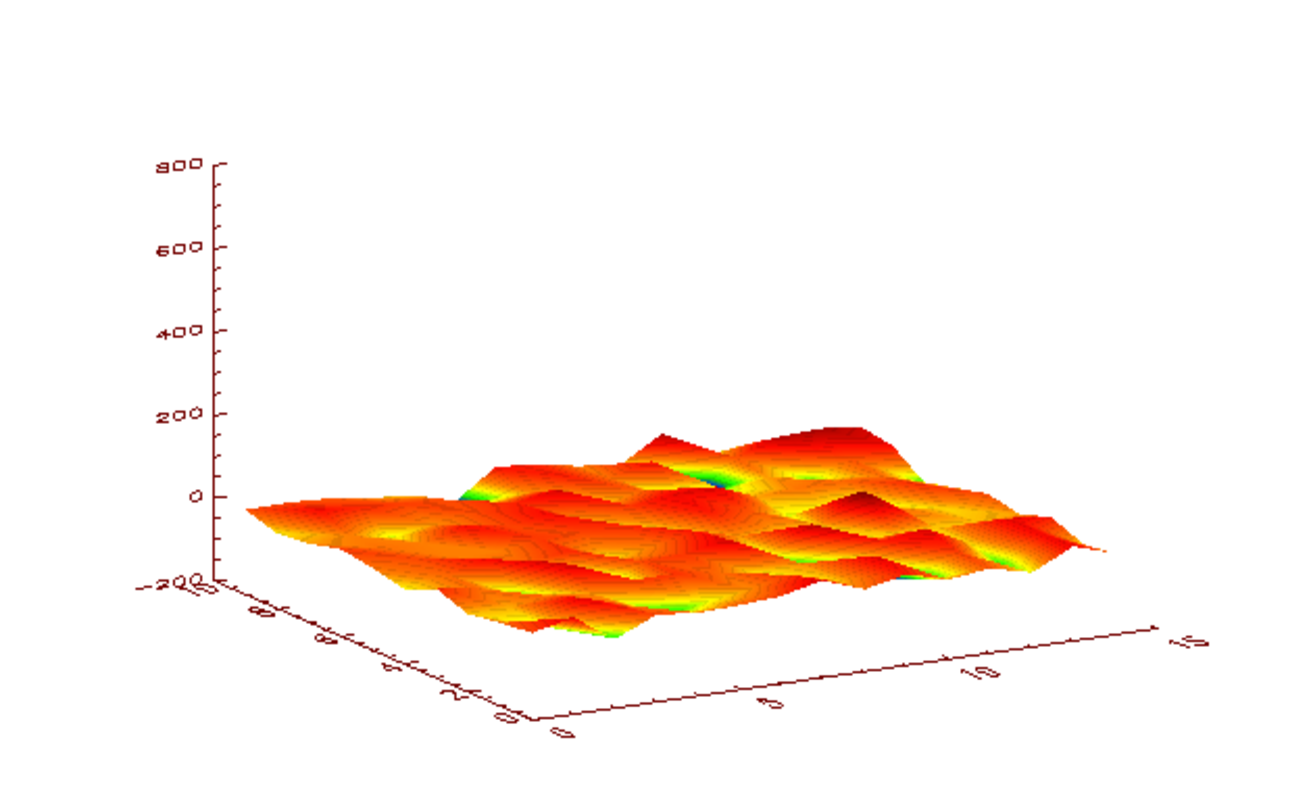
\includegraphics[width=9.3cm]{assets/figures/exempleResidu.pdf}
   \caption{De haut en bas : données, modèle, résidu = données - modèle.}
   \label{fig:dmr}
\end{figure}

\newpage

%----------
\section{Exercices du chapitre 9}
%----------

\begin{center}
\Large \bf {\underline{Pour faire ces exercices, utilisez \texttt{matlab}}}
\end{center}

%..........
\subsection*{Exercice 9.1 - corrélation linéaire, mesure d'une résistance électrique}
%..........

Lors d'une séance de travaux pratiques, les étudiants doivent mesurer la valeur d'une résistance $R$. Chaque étudiant dispose d'un voltmètre, d'un ampèremètre et d'une alimentation à courant continu. Un étudiant a obtenu les 5 mesures suivantes~:
\begin{center}
\begin{tabular}{r|ccccc}
U [V] & 0.204 & 1.23 & 2.04 & 3.48 & 4.83\\
I [mA] & 1.05 & 2.72 & 5.02 & 6.59 & 10.9
\end{tabular}
\end{center}

Ensuite, \textbf{à la main (c-à-d sans \texttt{Matlab}, mais avec une calculatrice scientifique)}, en utilisant les formules du cours,
\begin{enumerate}
\item calculez le coefficient de corrélation linéaire r;
\item déterminez les coefficients a et b de la droite de régression $\text{U}=\text{a}\,\text{I}+\text{b}$, en déduire la résistance R et l'offset $\text{U}_0$ éventuel;
\item refaites le calcul de la régression linéaire en posant $\text{b}=0$;
\item refaites le calcul de la régression en ajustant cette fois-ci le modèle \textbf{inverse} $\text{I}=\text{a}\,\text{U}+\text{b}$. Concluez.
\end{enumerate}

%..........
\subsection*{Exercice 9.2 - corrélation linéaire, test d'un modèle scientifique}
%..........

Dans le cadre d'un projet de recherche en instrumentation pour l'astrophysique, nous avons obtenu deux séries de mesures de la résolution angulaire à travers l'atmosphère terrestre turbulente, par deux moyens différents et totalement indépendants. Ces deux séries sont fournies dans le fichier \texttt{AngularResolutionSeries.txt}, sur \newline
\texttt{eistore1/profs/LJT/metrologie/cours/data...}. Lancez \texttt{Matlab} et chargez ces deux séries dans deux variables, $x$ et $y$.
\begin{enumerate}
\item calculez (à l'aide de \texttt{Matlab}) le coefficient de corrélation linéaire r des deux séries de mesures, \underline{en utilisant les formules du cours}; quelle est la qualité de la corrélation ? que peut-on en déduire sur ces deux méthodes de mesures de la résolution angulaires ?
\item calculez aussi, pour les deux séries, la valeur médiane et le mode.
\end{enumerate}

%..........
\subsection*{Exercice 9.3 - corrélation polynomiale}
%..........

Soit deux grandeurs physiques liées par la relation suivante~:
$$
y(x)=\exp{(a\,x^2+b\,x+c)}
$$
On a mesuré en laboratoire la série de 11 couples (x,y) suivante~:
\begin{center}
\begin{tabular}{r|ccccccccccc}
x & 0 & 0.1 & 0.2 & 0.3 & 0.4 & 0.5 & 0.6 & 0.7 & 0.8 & 0.9 & 1.0\\
y & 0.36 & 0.49 & 0.58 & 0.56 & 0.51 & 0.49 & 0.38 & 0.23 & 0.16 & 0.09 & 0.06
\end{tabular}
\end{center}
Linéarisez le modèle, puis faites un ajustement polynomial d'ordre 2, et calculez les coefficients a, b, et c qui réalisent le meilleur ajustement du modèle ci-dessus avec les mesures. Solution en l'absence d'erreurs de mesures~: $[a,b,c]=[-5,3,-1]$.

%..........
\subsection*{Exercice 9.4 - linéarisation d'un modèle exponentiel, régression linéaire}
%..........

Un biologiste a mesuré le nombre \underline{moyen} de bactéries encore actives en fonction de la durée d'un traitement chimique sur un substrat. Il a obtenu les résultats ci-dessous
\begin{center}
\begin{tabular}{r|ccccc}
durée $\Delta t$ [min] & 10 & 20 & 30 & 40 & 50 \\
nb. de bact. moyen & 1.893 & 0.970 & 0.511 & 0.215 & 0.137 \\
 & 60 & 70 & 80 & 90 & 100\\
 & 0.065 & 0.035 & 0.017 & 0.006 & 0.004
\end{tabular}
\end{center}
Le modèle associé à ces mesures est le suivant
$$
n(\Delta t)=n_0\,2^{-(\gamma\cdot\Delta t)}
$$
Faites la transformation qu'il faut sur $n(\Delta t)$ pour transformer cette expression ci-dessus en une relation linéaire du type $y=ax+b$, puis répondez aux questions suivantes
\begin{itemize}
\item quel est le coefficient de corrélation linéaire ? est-ce que le modèle en loi de puissance de 2 est un bon modèle ?
\item calculez les coefficients de la droite de régression
\item déduisez de ces coefficients les paramètres $n_0$ et $\gamma$ du modèle
\item quel est le nombre initial, a priori, de bactéries actives avant le traitement, c'est-à-dire pour $\Delta t=0$ ?
\item admettons que les spécifications de propreté pour les instruments chirurgicaux sont tels qu'il ne doit pas exister plus de 1 bactérie en moyenne pour 100 mm$^2$. Du modèle empirique que vous avez déduit des données, déterminez la durée de stérilisation nécessaire pour remplir cette spécification.
\end{itemize}

%..........
\subsection*{Exercice 9.5 - test de corrélation linéaire}
%..........

Les astrologues et autres charlatans aiment à dire qu'il existe une corrélation entre les phases lunaires et le nombre de naissances, afin de démontrer qu'il existe un lien entre les astres et les hommes (mais comme c'est chou !)

Lors d'une enquête dans un maternité, une statisticienne - quelqu'un de sérieux - à relevé les données suivantes
\begin{center}
\begin{tabular}{r|c|ccccccccc}
phase [\%] & $p$ & 0 & 12.5 & 25 & 37.5 & 50 & 62.5 & 75 & 87.5 & 100\\
nb. de naissances/jour & $n$ & 10 & 14 & 9 & 10 & 15 & 17 & 4 & 18 & 12
\end{tabular}
\end{center}
où la phase évolue entre 0 et 100 entre deux nouvelle Lunes consécutives, la phase de 50 \% correspondant à la pleine Lune.

Calculez le coefficient de corrélation linéaire entre la phase lunaire et le nombre de naissances. Concluez.

%..........
\subsection*{Exercice 9.6 - régression polynomiale}
%..........

\begin{center}
\begin{tabular}{c|ccccccc}
$x_i$ & -3 & -2 & -1 & 0 & 1 & 2 & 3\\
$y_i$ & -25 & 2 & 9 & 2 & -5 & 4 & 30
\end{tabular}
\end{center}
Ajustez le polynôme de 3-ème degré $$y(x)=a\,x^3+b\,x^2+c\,x+d$$ aux données ci-dessus.

%..........
\subsection*{Exercice 9.7 - régression générale}
%..........

Soit la fonction
$$
y(x)=a\,\cos{x}+b\,\sin^{2}{x}
$$
à ajuster sur la série de mesures suivante
\begin{center}
\begin{tabular}{c|ccccccccccc}
$x_i$ & 0 & 1 & 2 & 3 & 4 & 5 & 6 & 7 & 8 & 9 & 10\\
$y_i$ & 0.99 & 0.15 & -0.73 & -0.99 & -0.87 & -0.19 & 0.91 & 0.60 & -0.54 & -0.99 & -0.90
\end{tabular}
\end{center}
\begin{itemize}
\item développez toute la méthode analytique et construisez le modèle matriciel pour trouver les coefficient $a$ et $b$, à partir de la minimisation de l'écart quadratique entre le modèle est les données
\item appliquez la méthode aux données. La solution doit être proche de $[a,b]=[1,-0.5]$
\end{itemize}

\newpage

%..........
\subsection*{Exercice 9.8 - optimisation d'un processus}
%..........

\begin{wrapfigure}[13]{l}[0pt]{6cm}
	\centering
	\vspace{-5mm}
	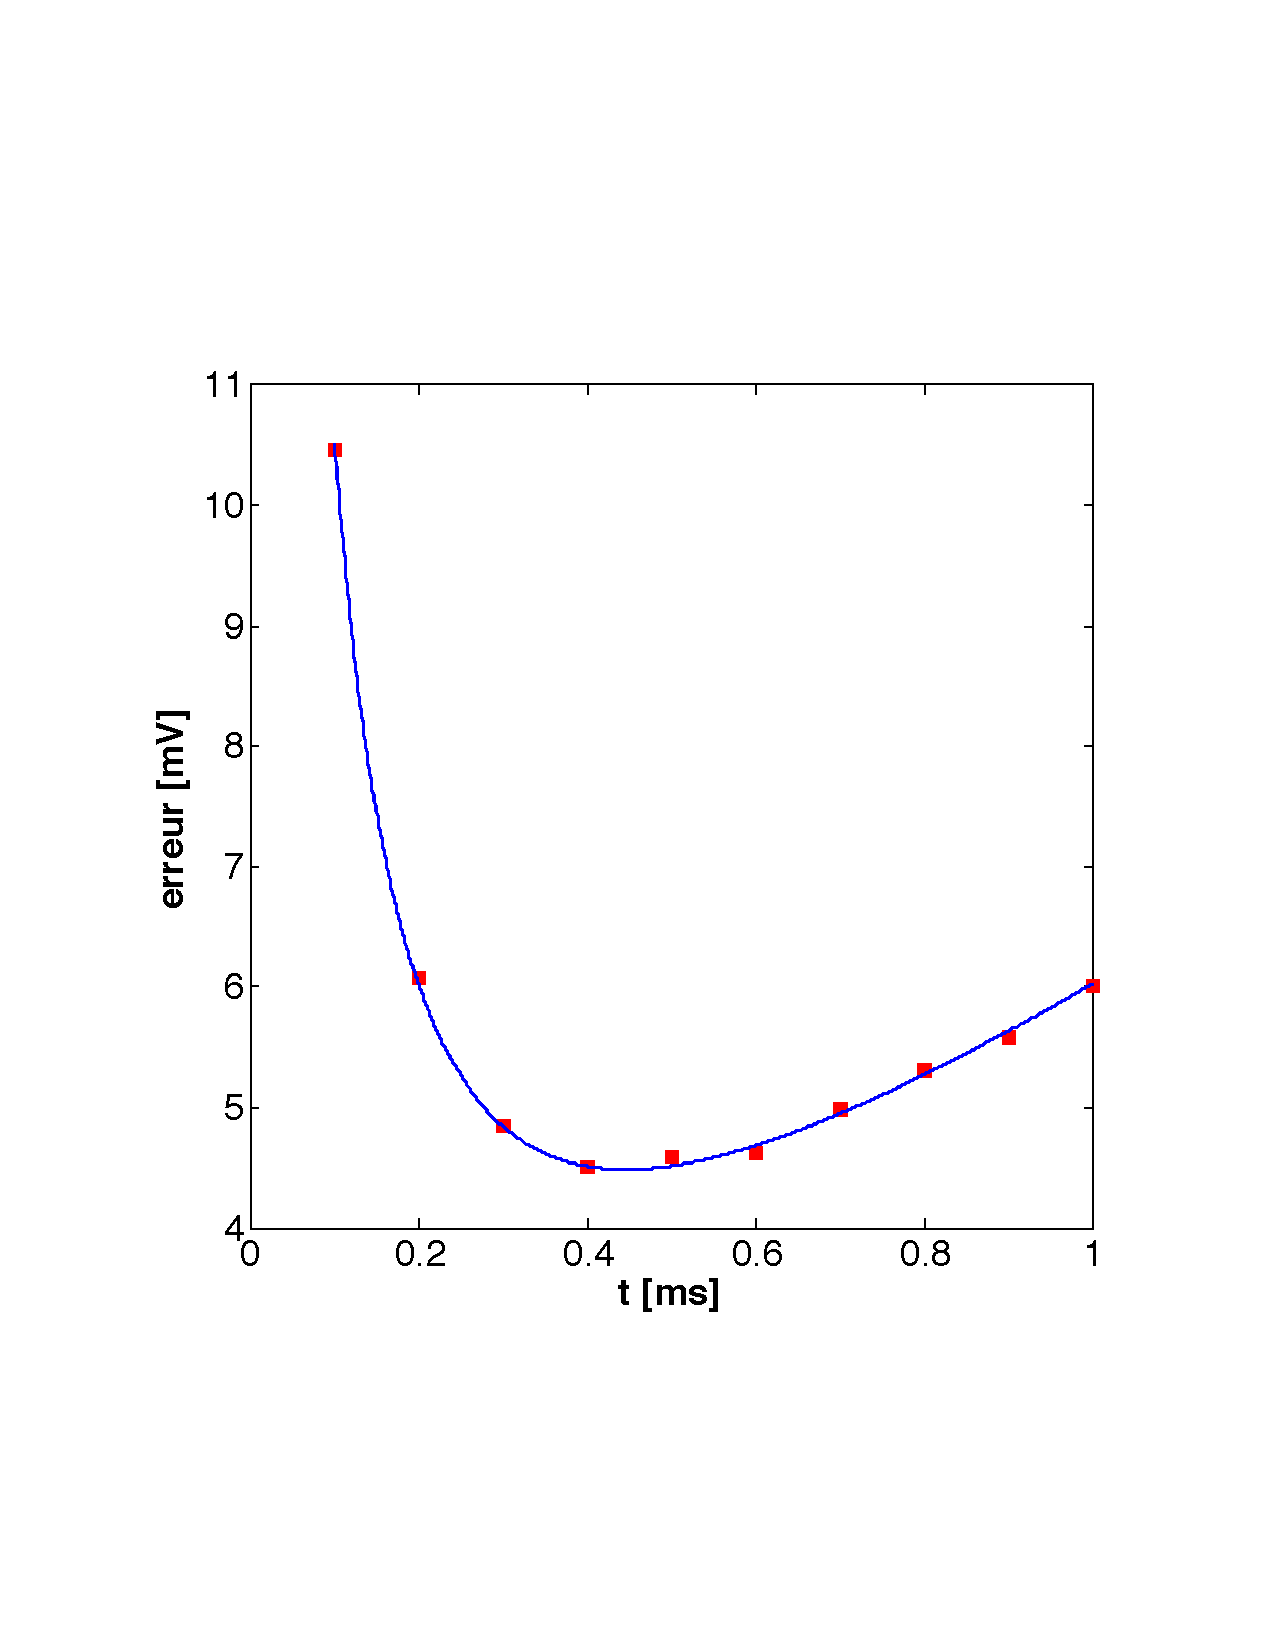
\includegraphics[width=6cm]{assets/figures/exe9fig1serie2.pdf}
	\caption{Mesures et modèle, exercice 8.}
	\label{fig:exe9}
\end{wrapfigure}
Imaginons un système asservi en tension électrique, dont la commande est perturbée par deux composantes : une erreur de retard pur, proportionnelle au pas d'horloge (inverse de la fréquence d'échantillonnage), et une erreur due au bruit de lecture du capteur, inversement proportionnelle au pas d'horloge. Le modèle de l'erreur totale sur la commande en fonction du pas d'horloge $\Delta t$ est le suivant
$$
\epsilon=a\,\Delta t+\frac{b}{\Delta t}
$$
Lors d'essais, on a mesuré l'erreur en fonction de $\Delta t$, et on a relevé les valeurs suivantes :
\begin{center}
\hspace{6cm}\begin{tabular}{r|cccccccccc}
$\Delta t_i$ [ms] & 0.1 & 0.2 & 0.3 & 0.4 & 0.5 \\
$\epsilon_i$ [mV] & 10.57 & 5.95 & 4.90 & 4.45 & 4.59 \\
                  & 0.6 & 0.7 & 0.8 & 0.9 & 1.0\\
                  & 4.64 & 4.87 & 5.20 & 5.63 & 5.99
\end{tabular}
\end{center}

Par ajustement du modèle, déterminez le pas d'horloge optimal, c'est-à-dire celui qui minimise l'erreur totale (faites tout d'abord un graphique des points de mesure, car il faut TOUJOURS examiner les données avant de les exploiter).